\chapter{Применение описанных подходов на практике}

В настоящей главе описывается эксперемент, в котором применялся
подход, описанный в главе~\ref{ch:problem_solving}, на
конкретной задаче определения демографических характеристик
пользователей с использованием конкретного набора данных.

В разделе~\ref{sec:dataset} произведён обзор набора данных,
который использовался в эксперименте, а также описана
конкретная задача, которая решалась.

В разделе~\ref{sec:algorithms_config} описаны применяемые
алгоритмы, а также их конфигурация.

В разделе~\ref{sec:result_quality} описан способ измерения
качества результата.

Наконец, в разделе~\ref{sec:results} приведены результаты,
полученные в результате проведения эксперимента.

\section{Описание набора данных}
\label{sec:dataset}

Для подтверждения состоятельности описанного подхода к решению задачи
профилирования пользователей на основе анализа их музыкальных
интересов был проведён эксперемент. Решалась задача определения
демографических характеристик (пола и возраста) пользователей сайта 
Last.fm с использованием набора данных, который использовался в
работе~\cite{wu2014gender}.

Авторы упомянутой работы загружали данные с сайта Last.fm. Всего набор
данных содержит 96807 пользовтель. Для каждого пользователя была
получена информация о его музыкальных интересах при помощи метода
публичного API сайта \textit{User.getTopTracks}, который возвращает
50 наиболее прослушиваемых музыкальных композиций заданным пользователем. 
Музыкальные композиции отсортированы в порядке убывания числа прослушиваний.
При этом данные содержат только имена исполнителей, извлечённые из этого списка.
То есть данные имеют такой вид, который был описан в 
разделе~\ref{sec:problem_formulation}. 

Кроме того, при помощи метода API сайта \textit{User.getInfo}
была получена информация о поле и возрасте для каждого пользователя.

Каждый пользователь в наборе описан по меньшей мере 40
музыкальными композициями. У каждого пользователя указан пол и возраст.
Набор данных содержит 133938 уникальных музыкальных исполнителей.

Стоит также отметить некоторые особенности выборки пользователей.
Во-первых, мужчин в ней содержится больше, чем женщин. Распределение
пола в выборке проиллюстрировано на рисунке~\ref{fig:gender_pie}.
Во-вторых, распределение возраста в выборке не является равномерным,
и оно смещено в сторону молодого поколения. Медиана распределения
возраста в выборке равна 31, а средний возраст равен 29,05.
Распределение возраста в выборке пользователей изображено на
рисунке~\ref{fig:age_histogram}.

Используя данные о музыкальных исполнителях пользователей,
решалось две задачи~--- задача определения пола и задача
определения возраста. Первая задача решалась как задача
бинарной классификации, а вторая~--- как задача восстановления
регрессии.

\begin{figure}[!h]
\caption{Распределение пола в выборке пользователей}
\label{fig:gender_pie}
\centering
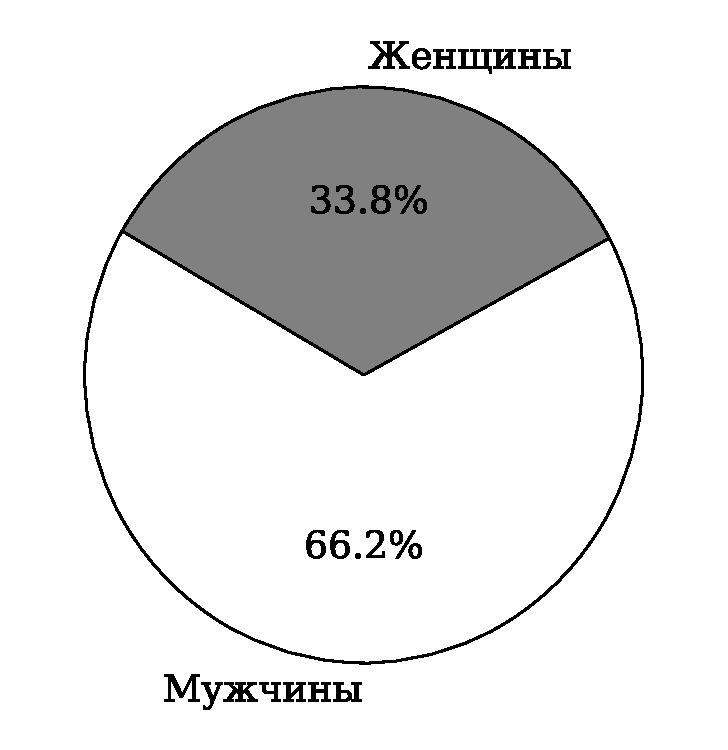
\includegraphics[scale=0.65]{figs/gender-pie.pdf}
\end{figure}

\begin{figure}[!h]
\caption{Распределение возраста в выборке пользователей}
\label{fig:age_histogram}
\centering
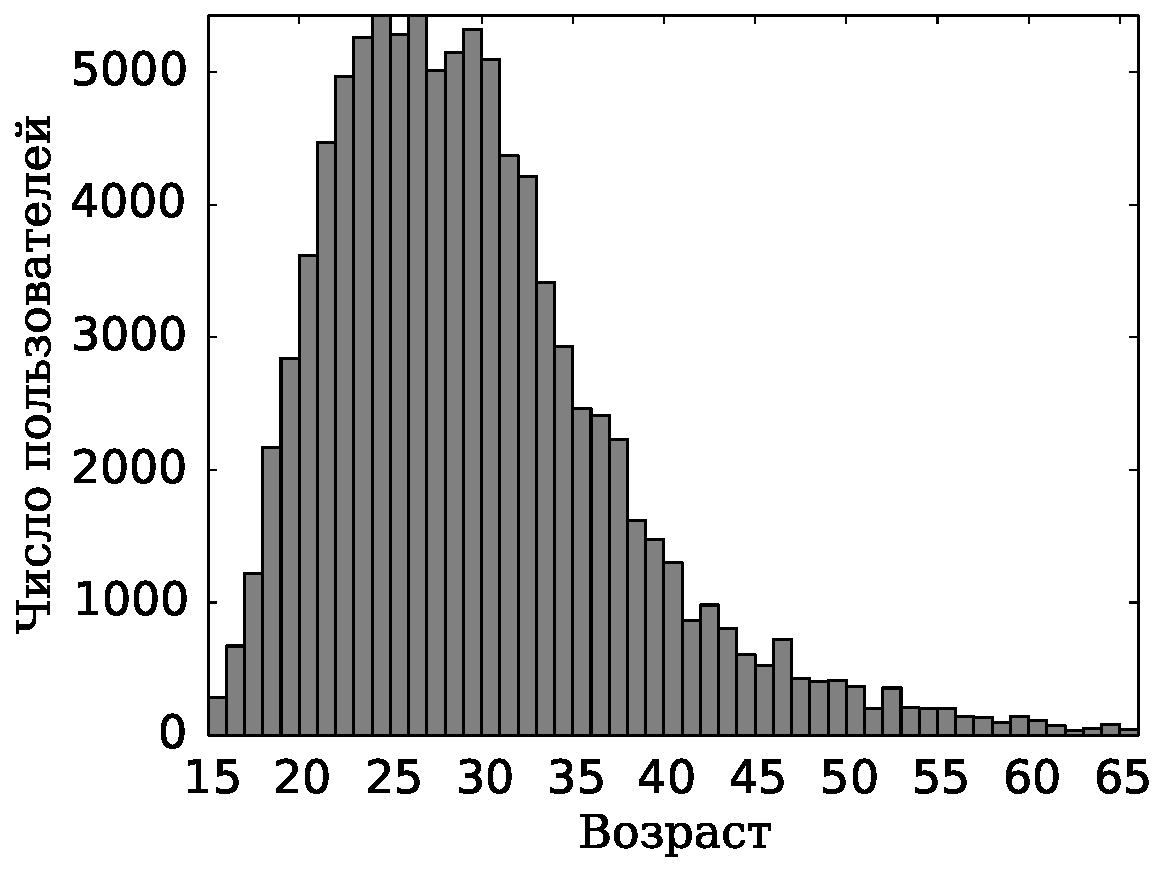
\includegraphics[scale=0.60]{figs/age-histogram.pdf}
\end{figure}

\section{Используемые алгоритмы и их конфигурация}
\label{sec:algorithms_config}

В данном разделе описаны используемые алгоритмы латентного
семантического анализа, техники word embedding, а также методов
классификации и восстановления регрессии. Кроме всего, приведены
конфигурации алгоритмов.

\subsection{Алгоритмы латентного семантического анализа}

В качестве алгоритмов латентного семантического анализа
в эксперименте использовались алгоритмы PLSA (реализация из библиотеки
\textit{BigARTM}~\cite{bigartm}), LDA (реализция из библиотеки
\textit{gensim}~\cite{gensim}) и LSI (реализация из библиотеки
\textit{gensim}).

Стоит отметить, что при использовании алгоритмов
\textit{PLSA} и \textit{LDA} результаты получались похожими 
на случайные, поэтому детальные эксперементы с их 
использованием не проводились. 

Возможно, такое поведение объясняется тем фактом, 
что их использование основано на гипотезе о существовании 
латентных жанров исполнителей, но часто не существует единогласного 
мнения о жанрах, которые исполняет тот или иной музыкальный исполнитель.
Поэтому можно считать, что данная гипотеза не выполняется.

Также имеет место предположение о том, что в большинстве случаев
люди предпочитают слушать музыку различных жанров, поэтому жанры
являются неинформативными признаками.

Напротив, использование алгоритма \textit{LSI} позволяет получить хорошие
результаты. Именно он и использовался в детальных экспериментах.

В качестве числа тематик в алгоритме \textit{LSI} использовалось
два значения~--- 200 тематик и 20 тематик. 
Для остальных параметров алгоритма использовались значения по умолчанию.

\subsection{Алгоритмы векторного представления слов}

В качестве алгоритма, реализующего модель векторного представления
слов использовался алгоритм Word2Vec, именно его реализация из
библиотеки \textit{gensim}.  

В качестве размерности векторов использовалось два значения~--- 200
и 20 (параметр \textit{size}).

Шириной контекста было выбрано значение 50 (параметр \textit{window}),
что означает использование в качестве контекста всех исполнителей для
любого из пользователей.

Для остальных параметров алгоритма Word2Vec использовались значения
по умолчанию.

\subsection{Алгоритмы классификации и восстановления регрессии}

В качестве алгоритма классификации или восстановления регресии
использовался \textit{метод опорных векторов (Support Vector Machine,
SVM)}~\cite{cortes1995support} с ядром 
\textit{radial basis function (RBF)}. Использовалась реализация
метода опорных векторов из программной библиотеки 
\textit{scikit-learn}~\cite{sklearn}, а именно алгоритмы
\textit{SVC} и \textit{SVR} для задач классификации и регрессии
соответственно.

Параметры метода опорных векторов \textit{C} и \textit{gamma},
выбор которых во многих задачах сильно влияет на результат,
настраивались на обучающей выборке (подробнее о разбиении
на обучающую и контрольную выборку см.
раздел~\ref{sec:result_quality}) методом \textit{GridSearchCV},
который реализован в библиотеке \textit{scikit-learn}. Множества
параметров \textit{C} и \textit{gamma} были выбраны следующие:
\[
    C \in \{0; 1; 0.5; 1; 3\},\quad
    \mathrm{gamma} \in \{0.001; 0.01; 0.1; 1; 8; 16; 32; 64\}.
\]
Обучающая выборка при настройке параметров разбивалась на три
части: две части для обучения, одна~--- одна для тестирования.

Для задачи определения пола параметры подбирались таким
образом, чтобы максимизировать точность классификации. 

Для задачи определения возраста параметры подбирались так, чтобы
минимизировать среднюю абсолютную ошибку (подробнее см.
раздел~\ref{sec:result_quality}).

\section{Способ измерения качества результата}
\label{sec:result_quality}

\section{Результаты}
\label{sec:results}

\chapterconclusion

Выводы выводы выводы
